\chapter{Aktueller Stand der Forschung und Praxis (generell auch wiedergeben von aktuell existierenden Lösungsmustern)}

\section{Ressourcenverbrauch bei KI-Modellen}
\subsection{Ressourcenverbrauch bei KI-Modellen}
\subsubsection{Nachhaltigkeit}
\subsubsection{Stromverbrauch}
\subsubsection{Rechenleistung begrenzt, KI-Modelle wachsen schneller als verfügbare Leistung}

\section{Deep Neural Network - Boltzmann Maschinen (Erstmal DNN erklären generell)}
\subsection{Konzept und Anwendung des Modells }

Eine \ac{BM} ist ein symmetrisches energiebasiertes Netzwerk bestehend aus Neuronen.\Footcite[Vgl.][260]{amariInformationGeometryBoltzmann1992}
Die Verbindung zwischen den einzelnen Neuronen werden dabei als bidirectional bezeichnet, da jedes Neoron in beide Richtungen miteinander kommuniziert.\footcite[Vgl.][149]{ackleyLearningAlgorithmBoltzmann1985}
Dabei ist die \ac{BM} ein zweischichtiges Modell und besitzt eine sichtbare Schicht (visible layer, ``v'') und eine verteckte Scicht (hidden layer, ``h'').\footcite[Vgl.][448]{salakhutdinovDeepBoltzmannMachines2009}
Das Netzwerk kann die Gewichte ``W'', die zwischen den Neuronen bestehen, durch spezifische Trainingsregeln updaten, basierend auf den Beobachtungen die als Input dienten.\footcite[Vgl.][1-2]{barraEquivalenceHopfieldNetworks2012}

\large Bild einfügen von einer Generellen Boltzmann Maschine

\begin{figure}[H]
    \centering
    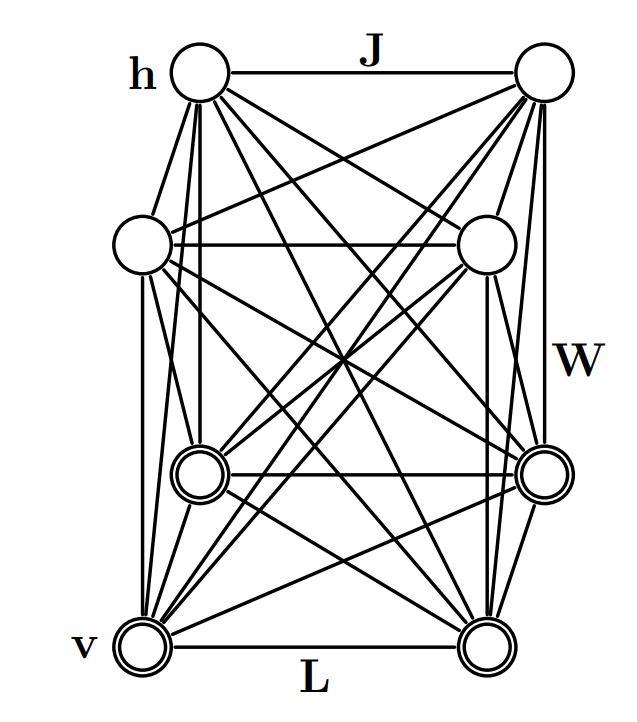
\includegraphics[width=0.3\linewidth]{graphics/General_BM.png}
    \caption{Visualisierung einer Generellen \ac{BM}\footcite[Vgl.][449]{salakhutdinovDeepBoltzmannMachines2009}}
\end{figure}

Schon 1985 war einem dem Gründervater für Künstliche Intelligenz, ``Geoffrey Hinton'', bewusst, dass eine \ac{BM} in der Lage ist, durch das Ansehen von Daten aus einem Bereich dessen zugrundeliegende Beschränkungen(Features) zu erlernen und ein generatives internes Modell zu entwickeln.\footcite[Vgl.][148]{ackleyLearningAlgorithmBoltzmann1985}
In einem Nächsten Schritt ist es somit möglich Beispiele mit derselben Wahrscheinlichkeitsverteilung wie die gezeigten Beispiele zu erzeugen.



\subsection{Energiefunktion}
\subsection{Training von BMs}
\subsubsection{Markov-Chain-Monte-Carlo-Verfahren}
Metropolis Hastings 
Conrtrastive Divergence

\subsection{Aktuelle Probleme mit RBM/BM}



\section{Hardwarebeschleuniger}
\subsection{Aktuelle Ansätze im Bereich KI und weitere Lösungen}
\subsubsection{Asics}
\subsubsection{Quantencomputing}
\subsection{ISING Maschine/ Physikinspirierter Hardwarebeschleuniger}
\subsubsection{Konzept (mit Energiefunktion), Probleme der Digitalrechner bzw. Unterschied zu Digitalrechner}
\subsubsection{Aktuelle Anwendung}
\subsubsection{Potentielle Einsatzgebiete für KI-Modelle}
\subsubsection{Parallelen Energiefunktion BM und ISING Maschine}

\section{Memristor Hopfield Network}
\subsection{Memristor}
\subsection{Hopfield Network}
\subsection{Crossbar}
\subsection{Output Hopfield Networtk}
\subsection{Noisy HNN}
